%%
%% Class homework & solution template for latex
%% Alex Ihler
%%
\documentclass[twoside,11pt]{article}
\usepackage{amsmath,amsfonts,amssymb,amsthm}
\usepackage{graphicx,color}
\usepackage{verbatim,url}
\usepackage{listings}
\usepackage{upquote}
\usepackage[T1]{fontenc}
%\usepackage{lmodern}
\usepackage[scaled]{beramono}
%\usepackage{textcomp}

% Directories for other source files and images
\newcommand{\bibtexdir}{../bib}
\newcommand{\figdir}{fig}

\newcommand{\E}{\mathrm{E}}
\newcommand{\Var}{\mathrm{Var}}
\newcommand{\N}{\mathcal{N}}
\newcommand{\matlab}{{\sc Matlab}\ }

\setlength{\textheight}{9in} \setlength{\textwidth}{6.5in}
\setlength{\oddsidemargin}{-.25in}  % Centers text.
\setlength{\evensidemargin}{-.25in} %
\setlength{\topmargin}{0in} %
\setlength{\headheight}{0in} %
\setlength{\headsep}{0in} %

\renewcommand{\labelenumi}{(\alph{enumi})}
\renewcommand{\labelenumii}{(\arabic{enumii})}

\theoremstyle{definition}
\newtheorem{MatEx}{M{\scriptsize{ATLAB}} Usage Example}

\definecolor{comments}{rgb}{0,.5,0}
\definecolor{backgnd}{rgb}{.95,.95,.95}
\definecolor{string}{rgb}{.2,.2,.2}
\lstset{language=Matlab}
\lstset{basicstyle=\small\ttfamily,
        mathescape=true,
        emptylines=1, showlines=true,
        backgroundcolor=\color{backgnd},
        commentstyle=\color{comments}\ttfamily, %\rmfamily,
        stringstyle=\color{string}\ttfamily,
        keywordstyle=\ttfamily, %\normalfont,
        showstringspaces=false}
\newcommand{\matp}{\mathbf{\gg}}




\begin{document}

\centerline{\Large Homework 1}
\centerline{CS 274B: Spring \& 2016}
\centerline{\bf Due: April 15, 2016}

\section*{Problem 1: }

I will assume that each random variable had $d$ states.

\subsection*{Part A}

To satisfy W, we need $d^3$ parameters \\
To satisfy Z, we need $d^2$ parameters \\
To satisfy Y, we need $d$ parameters\\
For probabilities of X, we need $d-1$ parameters\\
Our total is thus
\[
\frac{d^4-1}{d-1} + d - 2
\]

\subsection*{Part B}

For each random variable, we need $d-1$ parameters. \\
They are all independent\\
Thus our total is just $4(d-1)$

\subsection*{Part C}

The variables $Z,W,X$ each need $d$ parameters\\
The variable $Y$ needs $d-1$ parameters\\
\\
Thus our total is $4d-1$

\subsection*{Part D}

To satisfy Z, we need $d^2$ parameters\\
For X and Y, we need $d-1$ parameters for each one\\
To satisfy W, we need $d$ parameters\\
Our total is thus $d^2 + 2d - 1$

\subsection*{Part E}

To satisfy W,Y,Z, we need $d$ parameters\\
To satisfy Z, we need $d-1$ parameters\\
Our total is $4d-1$ 

\subsection*{Part F}

To satisfy W,Y,Z, we need $d$ parameters\\
To satisfy Z, we need $d-1$ parameters\\
Our total is $4d-1$ 

\section*{Problem 2:}

\subsection*{Part A}
No\\
Knowing the value of $\textit{projector\_plugged\_in}$ will affect the value of $\textit{power\_in\_wire}$ and subsequent variables in the network, none of which are $\textit{Sam\_reading\_book}$\\
Further, the value of $\textit{Sam\_reading\_book}$ is conditioned on the value of $\textit{room\_light\_on}$\\
The variables $\textit{room\_light\_on}$ and $\textit{power\_in\_wire}$ are conditionally independent given $\textit{power\_in\_building}$

\subsection*{Part B}

No\\
Knowing that $\textit{screen\_lit\_up}$ is true means that the probability of $\textit{ray\_says\_screen\_is\_dark}$ is affected but no other variable ended up affected.

\subsection*{Part C}

No\\
Knowledge of $\textit{screen\_lit\_up}$ and $\textit{projector\_plugged\_in}$ affect subsequent variables in the network none of which are $\textit{Sam\_reading\_book}$

\subsection*{Part D}

If $\textit{lamp\_works}$ was observed, then we would update the probabilities for $\textit{projector\_lamp\_on}$\\
We would then have to update the probabilities for $\textit{screen\_lit\_up}$\\
This would cause us to update probabilities for $\textit{ray\_says\_screen\_is\_dark}$

\subsection*{Part E}

If we observe just $\textit{power\_in\_projector}$ then the same variables from Part D will have their probabilities changed.

\section*{Problem 3: }

\subsection*{Part A}

We need to solve the following
\[
p(0,0;\theta) + p(0,1;\theta) + p(1,0;\theta) + p(1,1;\theta) = 1
\]
This ends up being the following:
\[
exp(-A(\theta)) + exp(-A(\theta)) + exp(\theta_x - A(\theta)) + exp(\theta_x + \theta_{xy} - A(\theta)) = 1
\]
After doing some factoring
\[
\frac{exp(\theta_x) + exp(\theta_{xy} + \theta_x) + 2}{exp(A(\theta))} = 1
\]
After cross multiplying and solving for $A(\theta)$
\[
A(\theta) = log( exp(\theta_x) + exp(\theta_{xy} + \theta_x) + 2 )
\]

\subsection*{Part B}
After letting $\theta_{xy} = 1$ we have the following
\[
A(\theta) = log( exp(\theta_x) + exp(1 + \theta_x) + 2 )
\]
After some factoring
\[
A(\theta) = log( exp(\theta_x)(1 + exp(1) ) + 2 )
\]
\begin{figure}[h]
\centering
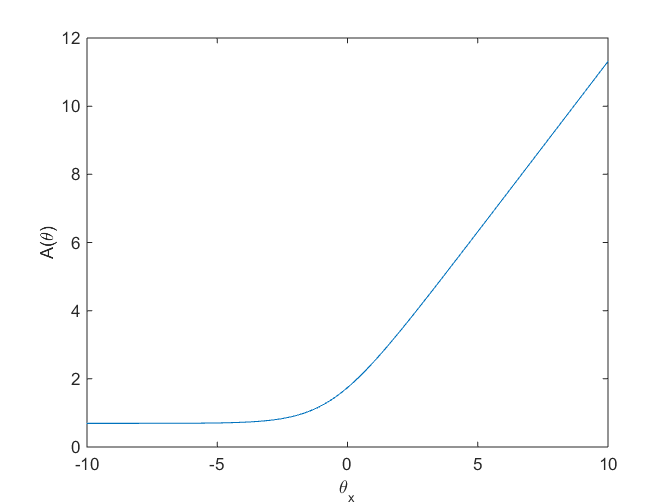
\includegraphics[width=4in]{prob3bplot.png}
\caption{Plot for $A(\theta)$. It appears convex as expected}
\end{figure}

\subsection*{Part C}
This is the partial with respect to $\theta_x$
\[
\frac{\partial A}{\partial \theta_x} = \frac{exp(\theta_x) + exp(\theta_x + \theta_{xy})}{exp(\theta_x) + exp(\theta_x + \theta_{xy}) + 2}
\]
This is the partial with respect to $\theta_{xy}$
\[
\frac{\partial A}{\partial \theta_{xy}} = \frac{exp(\theta_x + \theta_{xy})}{exp(\theta_x) + exp(\theta_x + \theta_{xy}) + 2}
\]
Thus we have 
\[
\bigtriangledown A(\theta) = [\frac{exp(1)+exp(3)}{exp(1)+exp(3)+2},\frac{exp(3)}{exp(1)+exp(3)+2}]
\]
Approximately 
\[
\bigtriangledown A(\theta) = [0.91937,0.80978]
\]
\end{document}
